\documentclass[tikz,border=2pt]{standalone}
\usepackage{amsmath,amssymb}
\usepackage{tikz}
\usetikzlibrary{arrows.meta}

\begin{document}
% A free variable x = x^+ - x^- with x^+, x^- >= 0: a positive value is carried by x^+, a
% negative value by x^-; in a basic solution at most one of the two is nonzero.
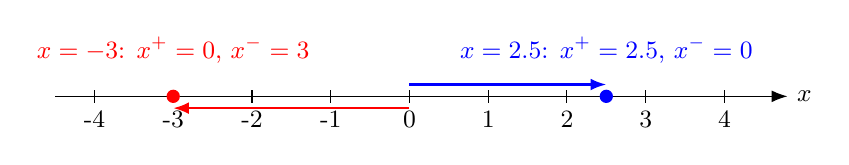
\begin{tikzpicture}[every node/.style={font=\small}, >={Latex[length=2mm]}]
	\draw[->] (-4.5,0) -- (4.8,0) node[right] {$x$};
	\foreach \v in {-4,-3,...,4} {\draw (\v,0.08) -- (\v,-0.08); \node[below=2pt] at (\v,0) {\v};}
	\fill[blue] (2.5,0) circle (2.4pt);
	\node[blue, anchor=south] at (2.5,0.3) {$x=2.5$: $x^+=2.5$, $x^-=0$};
	\draw[->, blue, thick] (0,0.15) -- (2.5,0.15);
	\fill[red] (-3,0) circle (2.4pt);
	\node[red, anchor=south] at (-3,0.3) {$x=-3$: $x^+=0$, $x^-=3$};
	\draw[->, red, thick] (0,-0.15) -- (-3,-0.15);
	\end{tikzpicture}
\end{document}
